\documentclass[letterpaper,11pt]{article}

\usepackage[margin=1.0in]{geometry}
\usepackage{amsmath}
\usepackage{amsthm}
\usepackage{amsfonts}
\usepackage{algorithm2e}
\usepackage{url}
\usepackage{fancyhdr}
\usepackage{blkarray}
\usepackage{graphicx}
\usepackage{csquotes}
\usepackage{cite}
\pagestyle{fancy}
\lhead{Algorithmic-Trading Summary --- Fall 2018}
\rhead{}


\begin{document}
\thispagestyle{plain}
\noindent{Algorithmic-Trading --- Fall 2018}

\noindent{Alex Thomas}

\noindent{Colgate University} \\

\noindent\textbf{Pairs Trading - Mean Reversion, Statistical Arbitrage }

\section*{Introduction }

Pairs trading is an algorithmic trading strategy that chooses two economically linked stocks and profits off the divergence in spread of prices. Pairs trading uses statistical arbitrage, which is attempted profit from pricing inefficiencies identified through mathematical models. The most basic assumption is that prices will move towards their historical average, which pairs trading takes advantage of.  However, unlike other instances of mean-reversion, this strategy has a distinct advantage of always being hedged against market movements. 

\section*{Motivations and Measures}

Pairs trading is motivated by statistical arbitrage and mean reversion\cite{Fu2009}. When given two stocks that are linked economically (i.e. Pepsi and Coca-Cola), we expect the spread to remain relatively constant over time. However, there might be divergence in the spread between these two pairs cause by factors such as supply/demand changes or changes in volume in a particular stock.  Another problem with this is finding stocks that are closely related. Because we need to have stocks that behave similarly, we use cointegration to identify pairs of similarly behaving stocks. 

\section*{Key Techniques}

This strategy is implemented by choosing and considering reasonably cointegrated pairs of stocks. Cointegration is a stationary measure that highlights horizontal trends \cite{Gatev2006}. Unlike correlation, which only tracks similarly moving magnitudes over time, it instead tells how the difference between two regression lines changes over time. The implementation uses the python extension statsmodels to generate the p-value for cointegration. It is absolutely key to have related stocks, as this strategy takes advantage of mean reversion, or in other words, stocks reverting back to their original mean in relation to other similarly behaving ones. Now this is quite difficult, as it is very difficult to find stocks that are behave very similarly. After running comparisons of cointegration, certain tech stocks such as INTC and MFST were found to behave similarly.  

To generate trading signals, a zscore is generated from the ratio of prices with the line of code: (ratios - ratios.mean())/ np.std(ratios). The zscore is a measure of how far away the current ratio of prices is away from its mean. Because of mean reversion, we can use this as a good indicator for buy and sell signals. A buy signal is generated when the zscore drops below -1, as we expect the zscore to return to its mean of 0. A sell signal is generated when the zscore goes above 1, as the stock is currently overvalued because we expect the stock to return to its mean of 0\cite{Fu2009}. In context of the pair of stocks, on buy signals the first stock in the pair is bought while the second is sold or shorted. The reverse is true on sell signals. 

\begin{figure}[ht!]
\centering
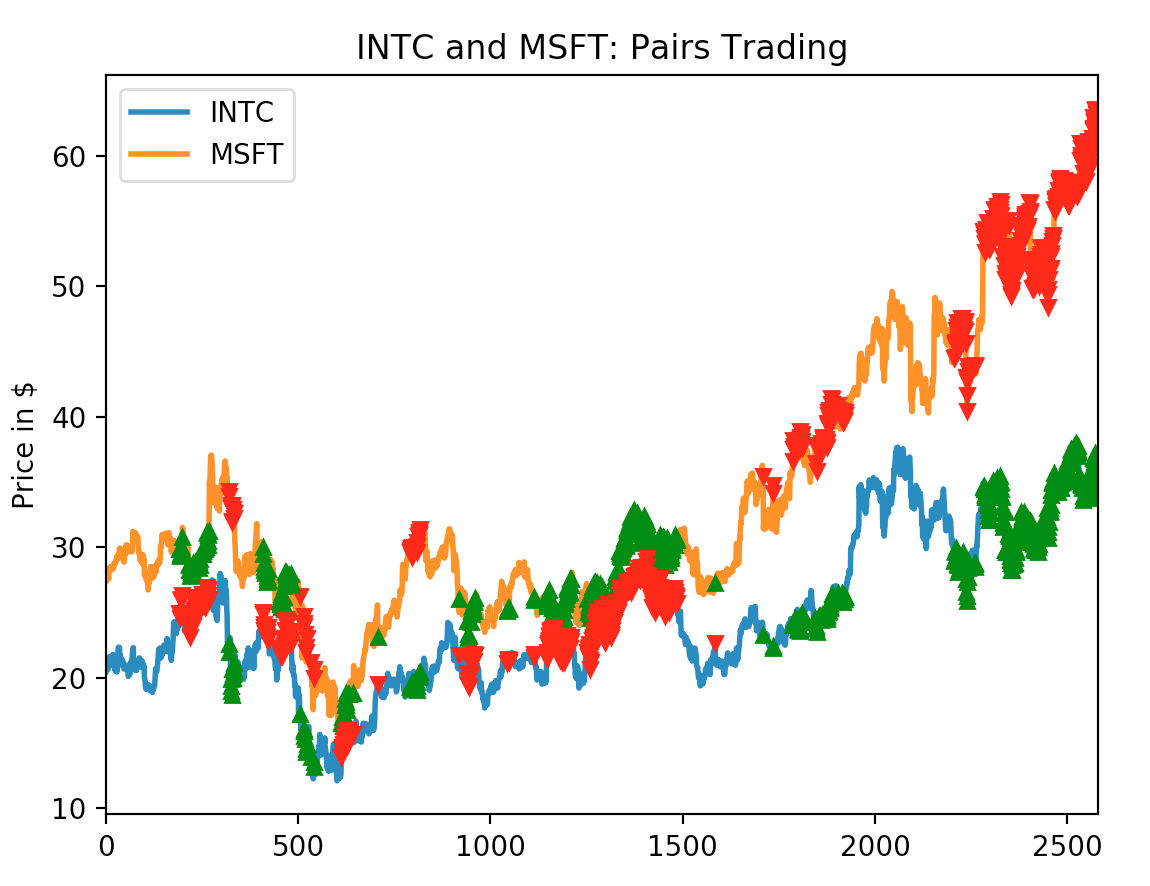
\includegraphics[width=90mm]{Intc_msft_signals.png}
\caption{Pairs Trading Strategy Applied to INTC and MSFT \label{overflow}}
\end{figure}

\begin{figure}[ht!]
\centering
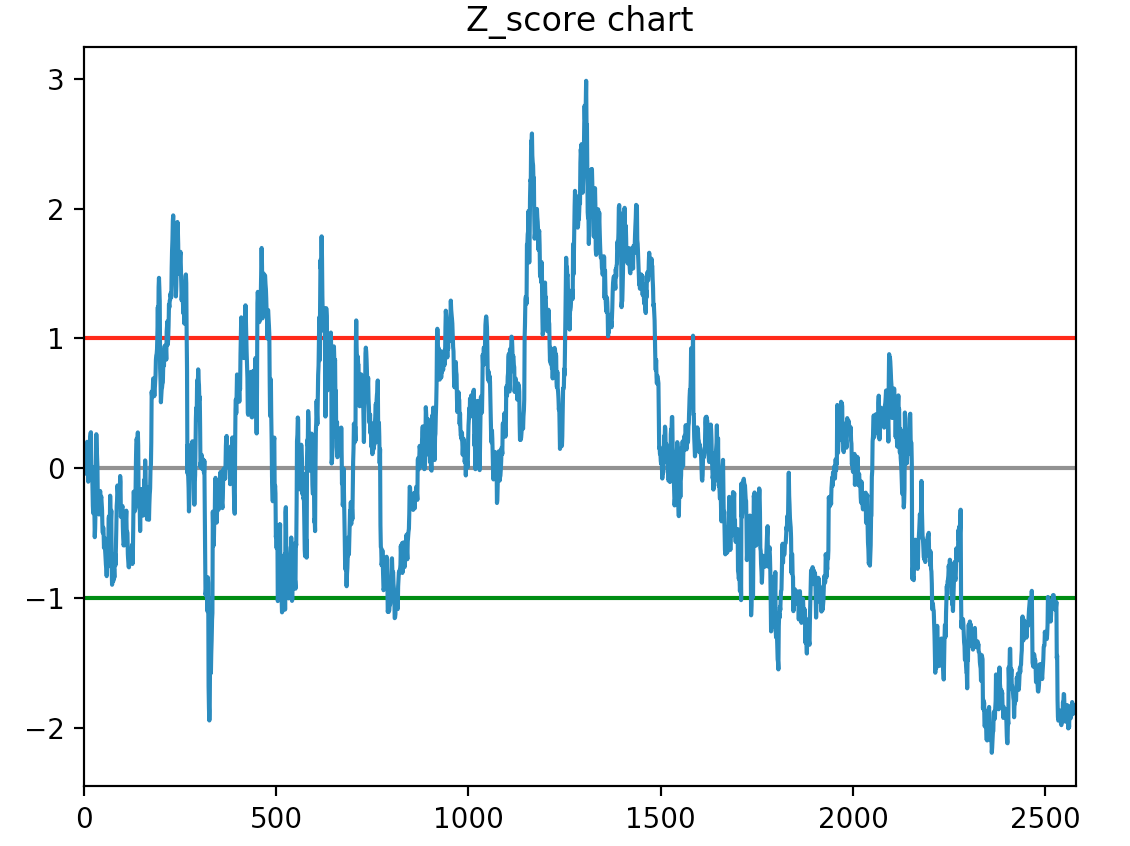
\includegraphics[width=90mm]{zscore.png}
\caption{Zscore of INTC and  MSFT \label{overflow}}
\end{figure}

\section*{Analysis}

\subsection*{Effectiveness}
This strategy takes advantage of mean reversion. Paired stocks are expected to have prices return back to the mean as they are expected to behave similarly. Because of this oppurtunity of arbitrage, we should expect this strategy to be very effective. However, it is important to note that pairs trading's effectiveness can be greatly diminished by high transactional cost \cite{Gatev2006}.

\subsection*{Runtime}
The components to consider for this strategy include pulling stock data into a Pandas data frame and calculating rolling means from the data-frame and marking their differences. Pandas is a python data analysis package and is perhaps the most powerful open source data analysis or manipulation tool available. For each calculation, it has to scrape through the entire data-frame at a rolling window, giving a linear runtime.

\subsection*{Quality Metric}
Unlike the previously implemented strategies, there were only 5 combinations of stocks that were reasonably cointegrated and produced reasonable p values of $< .05$ . The majority of combinations seemed to only be linked by stock performance and not any economic factors. A great example of linked stocks industry-wise is INTC and MSFT, which are shown in the above figures. What is interesting about this strategy is that it is very volume dependent. The implementation uses trades of sizes 10, 50, and 100 and tested against the benchmark of SPY, an industry standard for backtesting. As the volume of trades increases, so do returns. With trades of size 100, QCOM and SBUX pairs trading had returns of 363.77 \% and INTC and MSFT had returns of 225.89\%, absolutely crushing the benchmark return. However, the combination of AMD and EBAY were 27\% under the benchmark. The key to this strategy is volume and proper choice of paired stocks. When both of these is correct, the returns are truly spectacular.

\subsection*{Space / Memory Implications}
The only space for Pairs Trading required is the data-frame, which is very reasonable.

\section*{Conclusion}
Pairs Trading proves to be a very effective strategy given enough volume, which is more risky. However, our results show absolutely incredible profit levels with enough volume of trades to make this by far and away the most profitable strategy examined thus far. It would be interesting in the future to study an implementation where stocks are shorted instead of sold. 

\section*{Implementation}
\begin{verbatim}
def execute(stock1, stock2, start_date, end_date):
    stock_1 = stockDataRetriever(stock1, start_date, end_date).getStock()
    stock_2 = stockDataRetriever(stock2, start_date, end_date).getStock()

    # set Pandas df with both stocks
    df = pd.DataFrame(index=stock_1.index, stock_2.index)

    # create zscore from price ratios
    ratios = df['Close_stock1']/df['Close_stock2']
    zscore = (ratios - ratios.mean())/ np.std(ratios)

    # Create the buy and sell commands
    df['buy'] = np.where(zscore < -1, 1, 0)
    df['sell'] = np.where(zscore > 1, -1, 0)
    df['signal'] = df['buy'] + df['sell']

    # when signal changes from 1 to 0 or 0 to 1 - is a buy or sell
    df[positions] = df[signal].diff()

\end{verbatim}

\bibliographystyle{plain}
\bibliography{References}

\end{document}